\documentclass{article}

\usepackage{graphicx}
\usepackage{tikz}
\usepackage{tikzsymbols}
\usetikzlibrary{calc,patterns,shapes.geometric}
\pagestyle{empty}
\usepackage[margin=0pt]{geometry}
\geometry{papersize={14in,12in}}

\def\centerarc[#1](#2)(#3:#4:#5){\draw[#1] ($(#2)+({#5*cos(#3)},{#5*sin(#3)})$) arc (#3:#4:#5);}

\begin{document}
	\begin{figure}
		\centering
		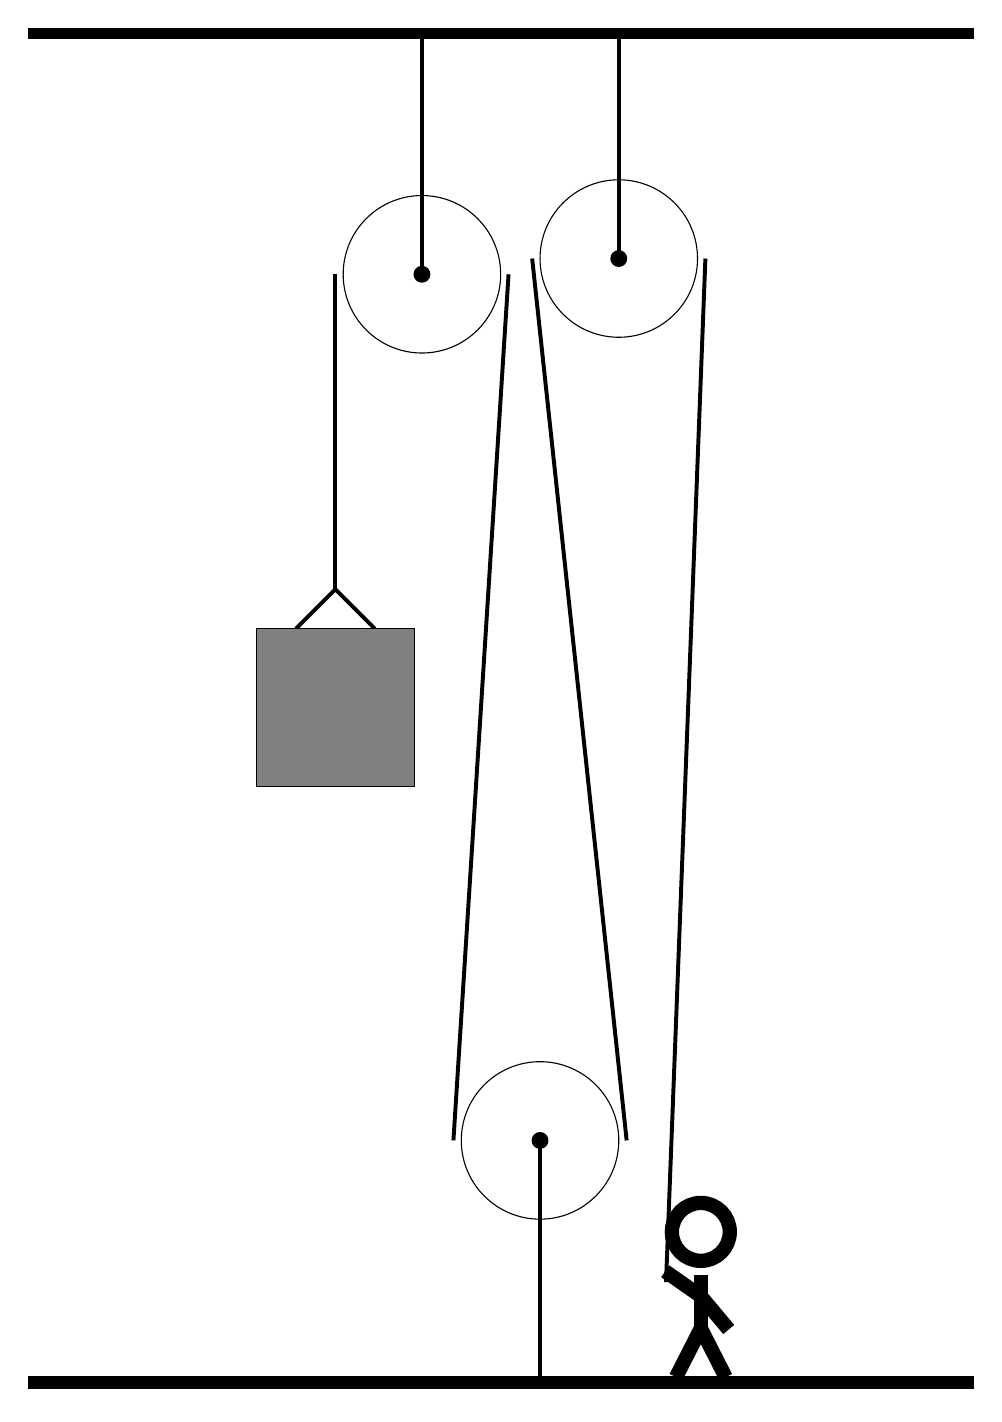
\begin{tikzpicture}
			%%%%% START %%%%%
			\draw[fill=black] (-4, 14) rectangle (8, 14.125);
			
			\draw (1, 11) circle (1);
			\draw[fill=black] (1, 11) circle (0.1);
			\draw[line width=0.5mm]  (1, 14) -- (1, 11);
			
			\draw[fill=white](2.5, 0) circle (1);
			\draw[fill=black] (2.5, 0) circle (0.1);
			\draw[line width=0.5mm]  (2.5, -3) -- (2.5, 0);
			
			\draw[fill=white](3.5, 11.2) circle (1);
			\draw[fill=black] (3.5, 11.2) circle (0.1);
			\draw[line width=0.5mm] (3.5, 14) -- (3.5, 11.2);
			
			\draw[line width=0.5mm] (-0.6, 6.5) -- (-0.1, 7.0) -- (0.4, 6.5);
			\draw[fill=black!50] (-1.1, 6.5) rectangle (0.9, 4.5);
			
			\draw[line width=0.5mm] (-0.1, 11) -- (-0.1, 7.0);
			\centerarc[line width=0.5mm](1, 11)(0:180:1.1);
			\draw[line width=0.5mm](2.1, 11) -- (1.4, 0);
			\centerarc[line width=0.5mm](2.5, 0)(180:360:1.1);
			\draw[line width=0.5mm](3.6, 0) -- (2.4, 11.2);
			\centerarc[line width=0.5mm](3.5, 11.2)(0:180:1.1);
			\draw[line width=0.5mm](4.6, 11.2) -- (4.1, -1.8);
			
			\node at (4.5, -1.9) {\Strichmaxerl[10][-35][-50]};
			
			\draw[fill=black] (-4, -3) rectangle (8, -3.15);
			%%%%% END %%%%%
		\end{tikzpicture}
	\end{figure}	
\end{document}